\documentclass[]{IEEEtran}
% some very useful LaTeX packages include:
%\usepackage{cite}      
\usepackage{graphicx}   
\usepackage{subfigure} 
\usepackage{url}       
\usepackage{amsmath}    
\usepackage{caption2}
% Your document starts here!
\begin{document}

% Define document title and author
	\title{Weekly Report}
	\author{Adviser: Prof. Yang Wen \\Student: Cheng Wensheng\\ Period: 2018.5.28-6.3
	}
	\markboth{Visual Information Processing Group}{}
	\maketitle

% Write abstract here
\begin{abstract}
	This week I mainly put my effort on practicing Pytorch and testing the new Titan V GPU. 
\end{abstract}

% Each section begins with a \section{title} command
\section{Pytorch practice}
	% \PARstart{}{} creates a tall first letter for this first paragraph
	\PARstart{T}{here} are many implementations about semantic segmentation frameworks with Pytorch. So I need to read them carefully and understand them totally, only by this way can we master Pytorch and implement my own networks as I want.
	\begin{itemize}
		\item I choose the FCN networks as my study object. Since it's the most classic networks and once I implement this, it's easier to transfer to following networks.
		\item The code mainly consists of 5 parts, including models, dataset, loss, metric and main. Fig.~\ref{fig:mp} is the overview of the Pytorch code. Fig.~\ref{fig:ss} is the training process of the semantic segmentation code with Tensorflow.
	\end{itemize}

% Main Part
\section{Titan V test}
	% LaTeX takes complete care of your document layout ...
	Since we got the new GPU, we try it on my server.
	\begin{itemize}
		\item About Pytorch, I tried a new code of StarGAN, a CVPR'18 oral paper, and I found that the training speed has been improved to be 2 times as the GTX1080. So the price is worthy.
		\item About Tensorflow, I tried the semantic segmentaiton framework with Tensorflow. But it seems that the training speed is almost the same as the before. Maybe it would be faster in the following versions of Tensorflow.
	\end{itemize}
\newpage
\begin{figure}[!hbt]
%		 Center the figure.
		\vspace{0.3cm}
%		\hspace{50cm}
		\begin{center}
			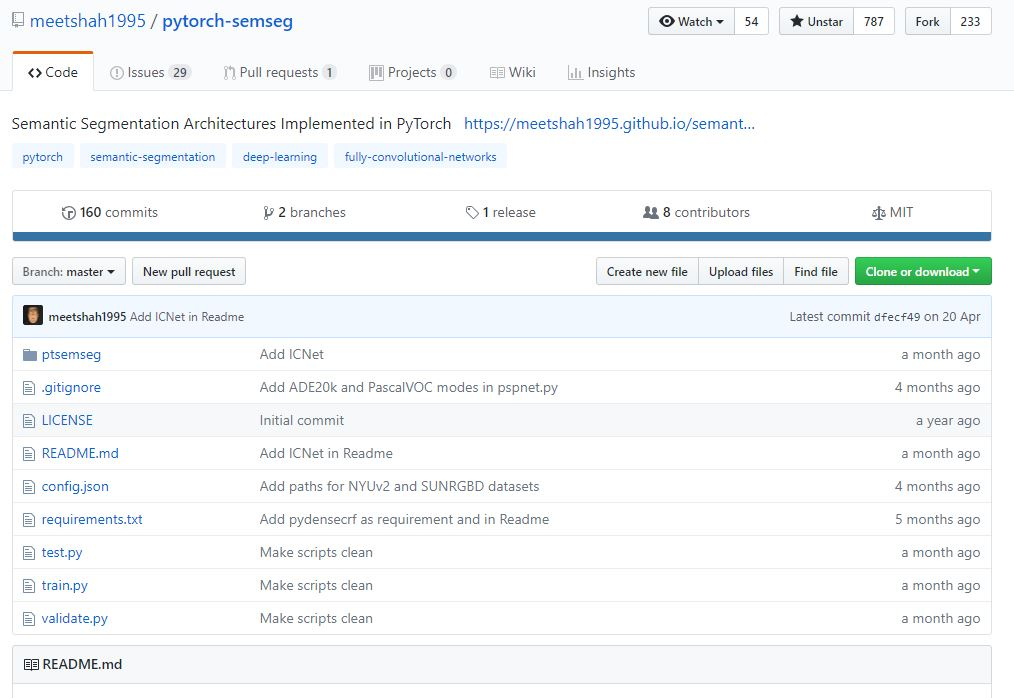
\includegraphics[width=\columnwidth]{code}
				%		 Create a subtitle for the figure.
			\caption{Code overview}
			\label{fig:mp}
		    \hspace{0.5cm}
			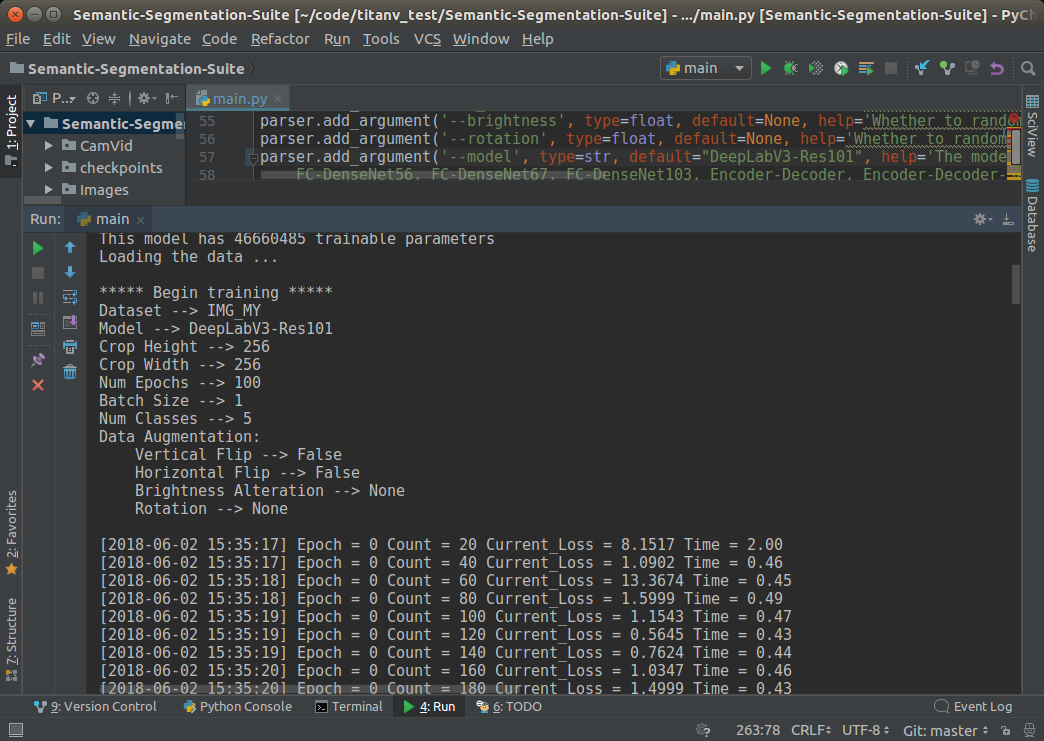
\includegraphics[width=\columnwidth]{record}
				%Create a subtitle for the figure.
			\caption{Semantic segmentation code with Tensorflow}
			\label{fig:ss}
		\end{center}
	\end{figure}

% Now we need a bibliography:
%\begin{thebibliography}{5}
%
%	%Each item starts with a \bibitem{reference} command and the details thereafter.
%	\bibitem{HOP96} % Transaction paper
%	J.~Hagenauer, E.~Offer, and L.~Papke. Iterative decoding of binary block
%	and convolutional codes. {\em IEEE Trans. Inform. Theory},
%	vol.~42, no.~2, pp.~429–-445, Mar. 1996.
%
%	\bibitem{MJH06} % Conference paper
%	T.~Mayer, H.~Jenkac, and J.~Hagenauer. Turbo base-station cooperation for intercell interference cancellation. {\em IEEE Int. Conf. Commun. (ICC)}, Istanbul, Turkey, pp.~356--361, June 2006.
%
%	\bibitem{Proakis} % Book
%	J.~G.~Proakis. {\em Digital Communications}. McGraw-Hill Book Co.,
%	New York, USA, 3rd edition, 1995.
%
%	\bibitem{talk} % Web document
%	F.~R.~Kschischang. Giving a talk: Guidelines for the Preparation and Presentation of Technical Seminars.
%	\url{http://www.comm.toronto.edu/frank/guide/guide.pdf}.
%
%	\bibitem{5}
%	IEEE Transactions \LaTeX and Microsoft Word Style Files.
%	\url{http://www.ieee.org/web/publications/authors/transjnl/index.html}
%
%\end{thebibliography}

% Your document ends here!
\end{document}